\input{preambulo.tex}

%----------------------------------------------------------------------------------------
%	TÍTULO Y DATOS DEL ALUMNO
%----------------------------------------------------------------------------------------

\title{	
\normalfont \normalsize 
\textsc{{\bf Ingeniería de Servidores (2015-2016)} \\ Grado en Ingeniería Informática \\ Universidad de Granada} \\ [25pt] % Your university, school and/or department name(s)
\horrule{0.5pt} \\[0.4cm] % Thin top horizontal rule
\huge Memoria Práctica 1 \\ % The assignment title
\horrule{2pt} \\[0.5cm] % Thick bottom horizontal rule
}

\author{Jorge Manuel Machado Cano} % Nombre y apellidos

\date{\normalsize\today} % Incluye la fecha actual

%----------------------------------------------------------------------------------------
% DOCUMENTO
%----------------------------------------------------------------------------------------

\begin{document}

\maketitle % Muestra el Título

\newpage %inserta un salto de página

\tableofcontents % para generar el índice de contenidos

\listoffigures

\listoftables

\newpage

\graphicspath{{./imagenes/}}

%----------------------------------------------------------------------------------------
%	Cuestión 1
%----------------------------------------------------------------------------------------

\section{Cuestión 1: ¿Qué modos y/o tipos de virtualización existen?}

\subsection{Hipervisor nativo o bare-metal (Tipo 1)}
Se llama hipervisor nativo a el sistema en el que el administrador de la máquina virtual controla directamente el hardware de la máquina, en vez de estar situado sobre una capa software (como un sistema operativo anfitrión). Este adminitrador se llama hypervisor. La principal característica de este tipo de virtualización es que el hipervisor se encarga de ceder recursos a cada uno de los sistemas operativos invitados, haciéndoles creer que poseen un hardware propio.\cite{hn}

\subsection{Hipervisor huésped (Tipo 2)}
Se llama hipervisor huésped al sistema en el que el administrador de la máquina virtual se encuentra sobre un sistema operativo anfitrión. De igual manera que el Tipo 1, este hipervisor coordina las llamadas al sistema de los sistemas operativos huésped y las ejecuta a través del sistema operativo anfitrión \cite{hh}

\subsection{Otros tipos de virtualización}
\begin{itemize}
\item Aplicaciones:
Ligado al concepto de aplicaciones portables como Java.
\item Memoria:
Consiste en hacer pensar a una aplicación que posee un espacio contiguo en una memoria RAM compartida.
\item Almacenamiento:
Consiste en abstraer la disposición del espacio físico en uno o varios espacios lógicos.
\end{itemize}


\section{Cuestión 2: Muestre los precios y características de varios proveedores de VPS (Virtual Private Server) y compare con el precio de servidores dedicados (administrados y no administrados). Comente diferencias.}
VPS de OVH: \cite{3}
\begin{itemize}
\item 4 cores 2.4/3.1 GHz
\item 8 GB RAM
\item 100 GB
\item 100 Mbps
\item 29,99 euros/mes
\end{itemize}

VPS de Arsys: \cite{4}
\begin{itemize}
\item 4 GB RAM
\item 100 GB SSD
\item 100 Mbps
\item 60 euros/mes
\end{itemize}

VPS de 1and1: \cite{5}
\begin{itemize}
\item 4 cores
\item 4 GB RAM
\item 300 GB
\item 100 Mbps
\item 30 euros/mes
\end{itemize}

Dedicado de 1and1: \cite{6}
\begin{itemize}
\item Intel®Xeon® E3-1270 V3
\item 16 GB RAM
\item 2 x 1.000 GB SATA GB
\item 100 Mbps
\item 79,99 euros/mes
\item Administrado por 10 euros al mes, incluye editor web, RSS, newsletter, administración de archivos y más características.
\end{itemize}

Dedicado de Arsys: \cite{7}
\begin{itemize}
\item Intel Xeon 4 core 2 GHz
\item 8 GB de RAM
\item 2 x 500 GB SATA
\item 100 Mbps
\item 125 euros/mes
\end{itemize}

Dedicado de OVH: \cite{8}
\begin{itemize}
\item Intel Xeon D D-1520
\item 128 GB RAM
\item 2 x 2 TB soft
\item 250 Mbps
\item 119,99 euros/mes
\end{itemize}

Podemos comprobar que los VPS son más caros que los servidores dedicados, esto se debe a que en un VPS se comparte máquina con el resto de usuarios, mientras que en un servidor dedicado la máquina solo pertenece a un usuario, lo que garantiza la disponibilidad de los recursos.


\section{Cuestión 3: ¿Qué otros software de virtualización existen además de VMWare y Virtual Box?}

\subsection{Windows virtual PC}
Tal como indica en \cite{9}: \\
\textit{"Windows Virtual PC es lo último en tecnología de virtualización de Microsoft. Esta tecnología se puede usar para ejecutar más de un sistema operativo a la vez en un equipo, así como muchas aplicaciones de productividad en un entorno virtual de Windows, con un solo clic y directamente desde un equipo en el que se ejecute Windows 7."} 

\subsection{Parallels}
Tal como indica en \cite{10} \\
\textit{"Parallels Desktop para Mac le permite ejecutar sin problemas y en paralelo las aplicaciones de Windows y Mac OS X Mountain Lion con rapidez, control y de forma segura."}

\subsection{QEMU}
QEMU es un software de virtualización libre genérico \cite{11}

\section{Cuestión 4: Enumere algunas de las innovaciones en Windows 2012 R2 respecto a 2008R2.}

Datos obtenidos en \cite{12}

\begin{itemize}
\item Control de acceso dinámico: Esto permite el control del acceso a los archivos y auditar quien ha accedido a ellos.
\cite{13}
\item Hyper-V Replica: Sistema que permite replicar una máquina virtual desde un servidor a otro servidor secundario manteniendo coherencia de los cambios producidos en la réplica.\cite{14}
\item Shared VHDX: Permite compartir discos duros entre máquinas virtuales de forma que no quede expuesta la topología de almacenamiento. \cite{15}
\item IP address management: se trata de un sistema utilizado para administrar el espacio de direcciones IP en una red corporativa. \cite{16}
\end{itemize}

\newpage

\section{Cuestión 5: ¿Qué empresa hay detrás de Ubuntu? ¿Qué otros productos/servicios ofrece?}

La empresa que se encuentra detrás de Ubuntu es Canonical \cite{17} \\
A parte de Ubuntu, Canonical ofrece herramientas para la creación, administración y escalado de servicios cloud, tales como Landscape, Juju o MAAS. Ofrece diferentes versiones de ubuntu para diferentes sistemas, como servidor, tablet y smartphone, además de la conocida versión Desktop. \cite{18}

\section{Cuestión 6: ¿Qué relación tiene esta distribución (CentOS) con Red Hat y con el proyecto Fedora?}
CentOS es un proyecto patrocinado por Red Hat desde 2014, compilado por voluntarios a partir de código fuente de Red Hat Enterprise Linux (en adelante RHEL) liberado con Licencia Pública General de GNU por Red Hat. \cite{19} \\
Fedora también es un proyecto derivado de RHEL, la principal diferencia se basa en que RHEL es comercial, por lo tanto está sujeto a distintas fases de prueba. \cite{20}

\section{Cuestión 7: Indique qué otros SO se utilizan en servidores y el porcentaje de uso.}

Según w3techs, que analiza los SO de sitios web el porcentaje es:
\begin{figure}[H]
\centering
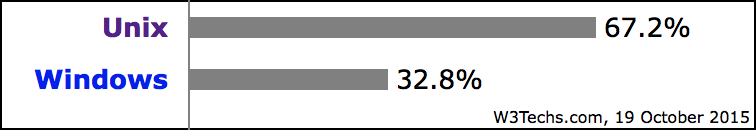
\includegraphics{w3tech1}
\caption{Porcentajes de uso de SO en servidores de páginas web.}
\cite{figura1}
\end{figure}

Dentro de Unix podemos distinguir entre:
\begin{figure}[H]
\centering
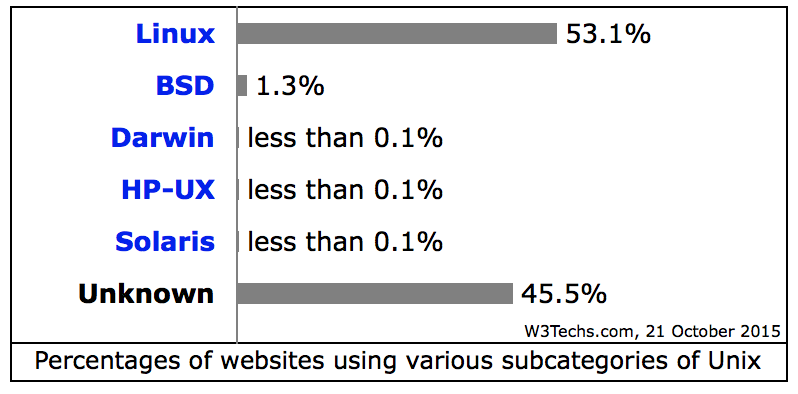
\includegraphics{w3tech2}
\caption{Porcentajes de uso de SO en servidores Unix de páginas web.}
\cite{figura2}
\end{figure}
Si tenemos en cuenta cualquier tipo de servidor (no solo de sitios web) la distribución es:
\begin{figure}[H]
\centering
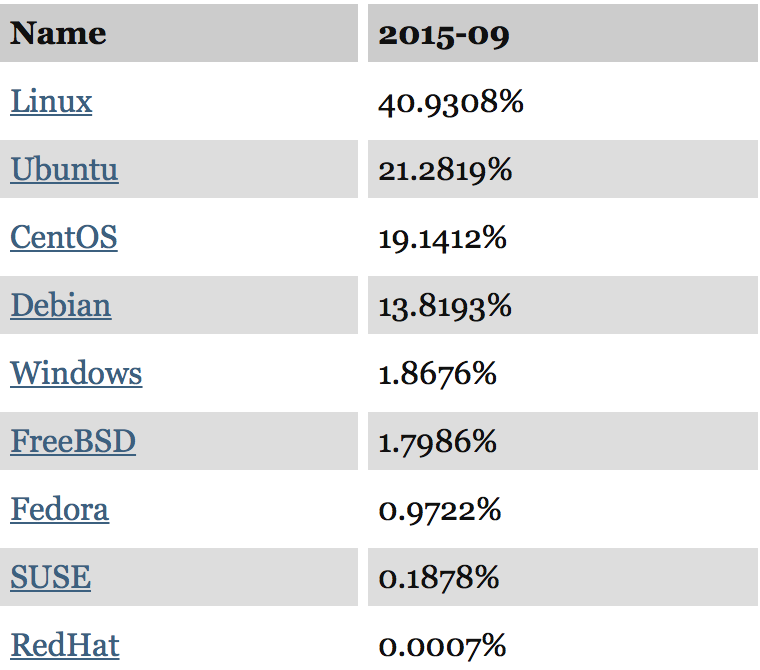
\includegraphics[scale=0.5]{w3tech3}
\caption{Porcentajes de uso de SO en servidores.}
\cite{figura3}
\end{figure}

\newpage

\section{Cuestión 8: ¿Qué diferencia hay entre RAID mediante SW y mediante HW?}

El RAID software aporta una carga extra al SO, ya que internamente se encarga de realizar los movimientos de datos necesarios, cosa que no ocurre mediante un RAID hardware, ya que éste está implementado en un circuito existente en la placa base, lo que no sobrecarga al software

\section{Cuestión 9: a) ¿Qué es LVM? b)¿Qué ventaja tiene para un servidor de gama baja? c) Si va a tener un servidor web, ¿le daría un tamaño grande o pequeño a /var?}

LVM es un gestor de volúmenes del kernel de linux\cite{21}, su función consiste en unir o separar el espacio físico de la máquina, como por ejemplo unir dos discos duros magnéticos en un solo espacio virtual, para posteriormete separar este espacio en volúmenes lógicos, pudiendo asignar cada uno de estos espacios a cada una de las carpetas principales de una sistema Linux, como root, home o var, permitiendo además que cada uno de estos volúmenes lógicos se formatee con un sistema de archivos distinto\cite{22}.\\
La principal ventaja de este sistema para un servidor de gama baja se basa en que utilizando un disco duro de gran capacidad, lo que supone un coste menor que varios discos pequeños, podemos ofrecer a nuestros clientes un disco duro lógico independiente del resto de los clientes. Este sistema también nos permitiría añadir nuevos discos duros al sistema de forma fácil y añadir más espacio a cualquiera de los clientes que lo solicite.

Es importante asignar un tamaño grande a /var en un servidor, ya que en este directorio se almacena gran cantidad de datos sobre el funcionamiento del sistema, usuarios y procesos, los llamados logs, archivos temporales grandes, o que necesitan estar más tiempo del permitido en el directorio /tmp. Este directorio también aloja bases de datos y archivos que utilizan los programas en funcionamiento.\cite{var}

\section{Cuestión 10: ¿Debemos cifrar también el volumen que contiene el espacio para swap? ¿y el volumen en el que montaremos /boot?}

Debemos cifrar swap, ya que como sabemos, en swap se aloja en contenido que debería estar en memoria principal pero que por cuestiones de falta de espacio físico no podemos almacenar en ella, por lo tanto el contenido se aloja en la partición swap del disco duro de la máquina. Si tenemos el resto del disco duro encriptado, cuando algún programa requiera algún dato en memoria principal deberá desencriptarlo, pero si el dato no cabe en memoria principal y es trasladado a swap, tal dato se encontrará desencriptado en el disco duro, por lo que el trabajo de encriptado/desencriptado de los datos habría sido inútil.\\
No es aconsejable encriptar boot si no queremos un sistema con la máxima seguridad, ya que en /boot se encuentran los archivos necesarios para el ararnque el sistema operativo, por lo que si estuviera encriptado necesitaríamos desencriptarlo con un dispositivo externo para arrancar nuestra máquina, como por ejemplo una unidad flash.

\section{Cuestión 11: ¿Qué otro tipo de usos de una partición le permite configurar el asistente de instalación? ¿Cuál es la principal diferencia entre ext4 y ext2?}

Nos permite utilizar ext4, ext3, ext2, btrfs, JFS, XFS, FAT16, FAT32, área de intercambio y volumen físico para LVM.

La principal diferencia es que ext4 cuenta con el sistema de journaling, esto evita la pérdida de información a la hora de la escritura, guardando la estructura de datos que vamos a modificar en un espacio reservado, y modificando la estructura de datos una vez el paso anterior se ha completado con seguridad. En caso de error (fallo de corriente, sistema operativo) tenemos una copia de seguridad para restaurar los datos. Esto provoca una pequeña sobrecarga.\cite{23}\\
Ext2 no cuenta con este sistema, lo que lo hace algo más rapido.

\section{Cuestión 12: Muestre cómo ha quedado el disco particionado una vez el sistema está instalado. (lsblk)}

\begin{figure}[H]
\centering
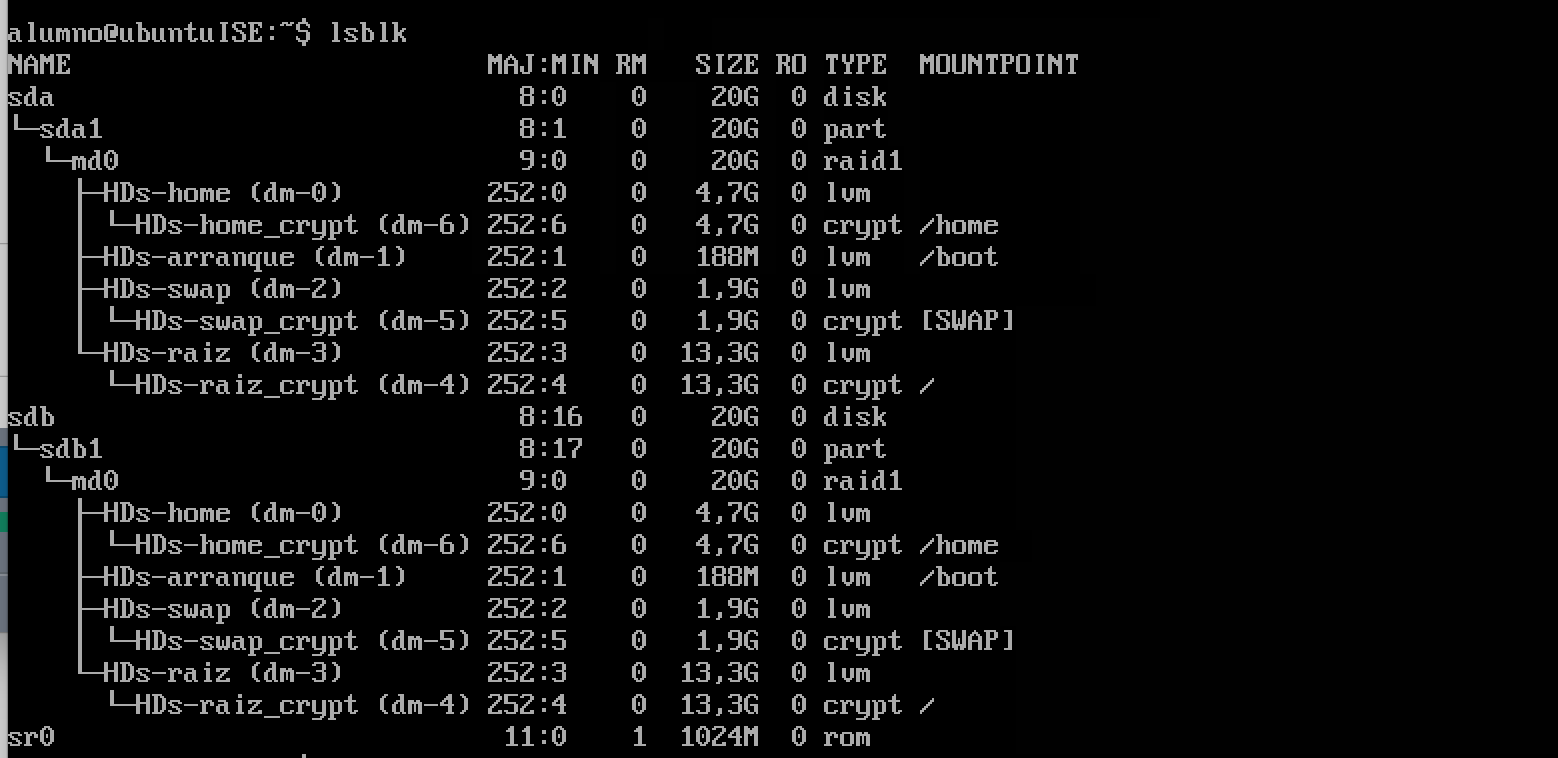
\includegraphics[scale=0.8]{lsblk}
\caption{Captura de pantalla de lsblk.}
\end{figure}

\section{Cuestión 13: a) ¿Cómo ha hecho el disco 2 “arrancable”? b) ¿Qué hace el comando grub-install? c) ¿Qué hace el comando dd?}
\subsection{a}
\begin{figure}[H]
\centering
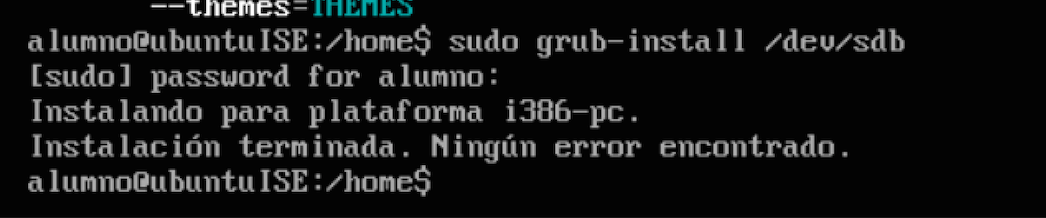
\includegraphics{grubinstall}
\caption{Comando para hacer el disco 2 “arrancable”.}
\end{figure}
\subsection{b}
Grub-install, según el manual de Linux, instala GRUB en cualquier dispositivo que se incluya en los argumentos, lo que lo convierte en booteable.
\subsection{c}
Según el manual de linux, la función del comando dd es copiar un archivo, convirtiendo y formateando los datos según los operandos, es capaz de obtener y exportar los datos desde flujos de entrada o de salida de bytes o desde archivos.

\section{Cuestión 14: ¿Qué diferencia hay entre Standard y Datacenter?}
Datacenter está orientado a entornos altamente virtualizados, mientras que el Standard no. \cite{24}

\section{Cuestión 15: Continúe usted con el proceso de defnición de RAID1 para los dos discos de 50MiB que ha creado. Muestre el proceso con capturas de pantalla.}
\begin{figure}[H]
\centering
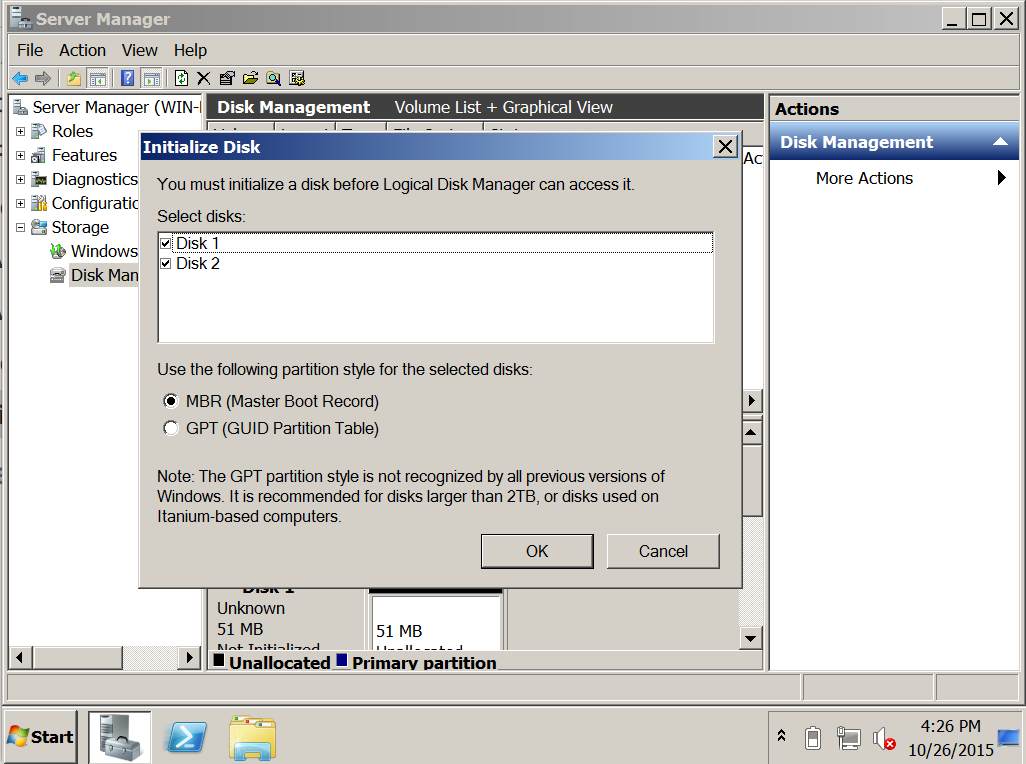
\includegraphics[scale=0.5]{raid1}
\caption{Esta ventana aparece al iniciar la gestión de discos, inicializamos ambos discos para que el administrador de discos lógicos pueda acceder a ellos.}
\end{figure}
\begin{figure}[H]
\centering
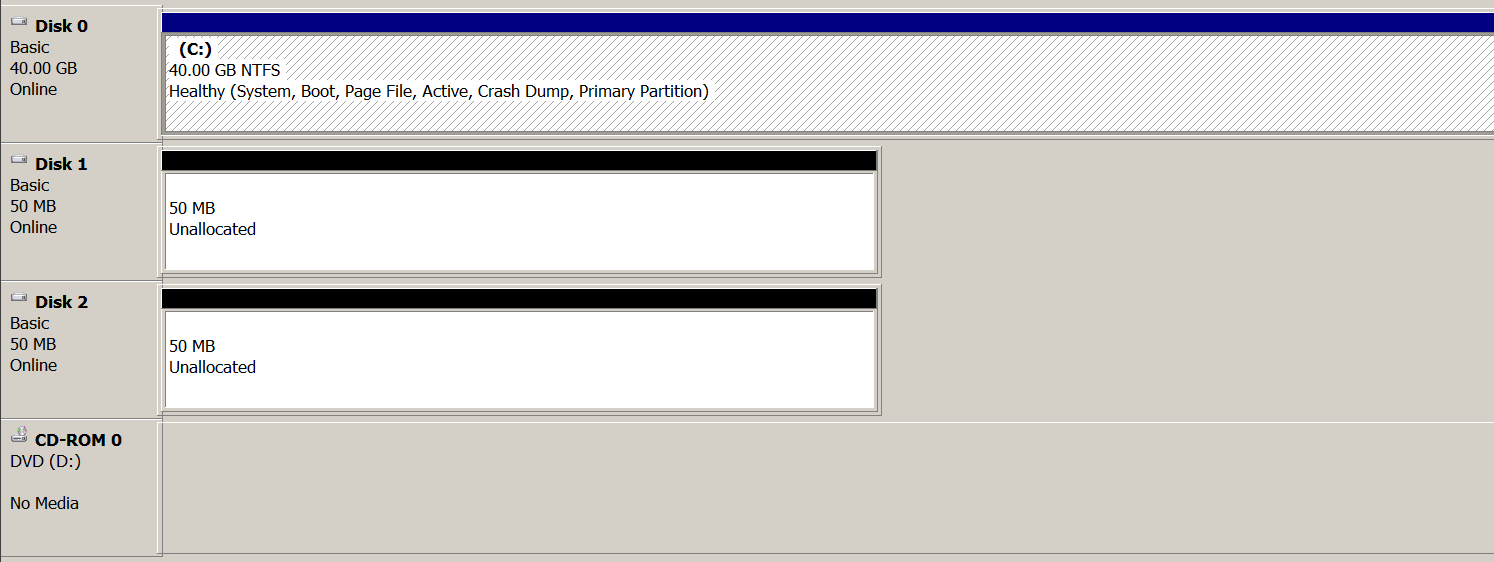
\includegraphics[scale=0.5]{raid2}
\caption{Como podemos comprobar, ambos discos están online.}
\end{figure}
\begin{figure}[H]
\centering
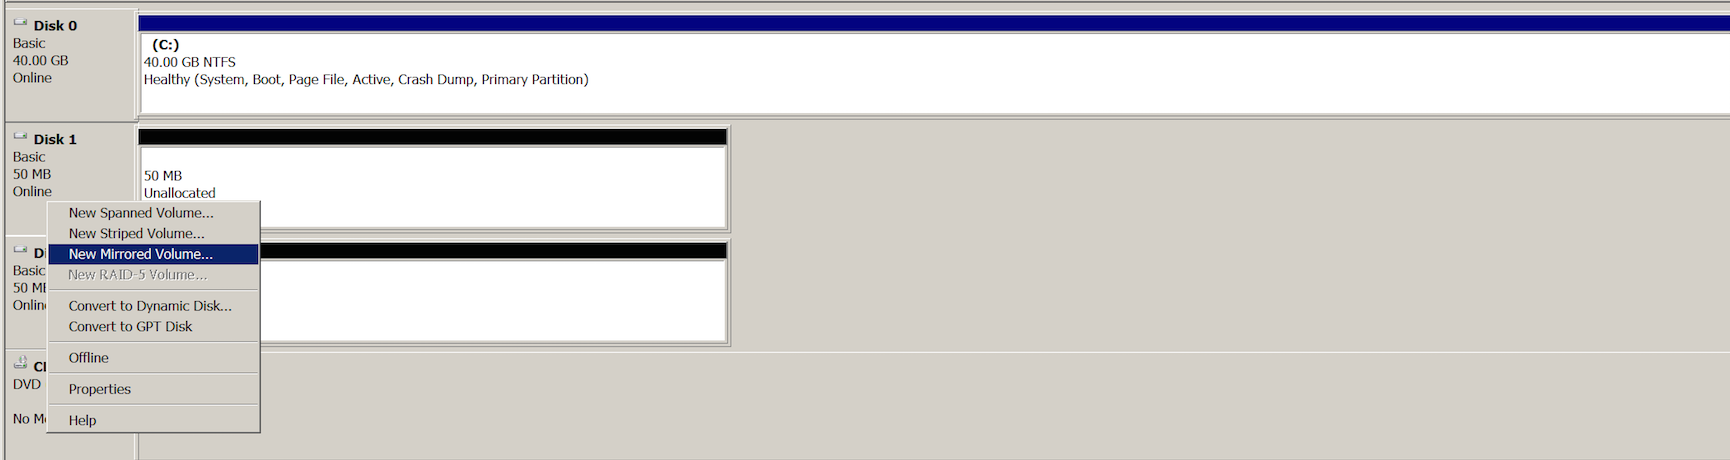
\includegraphics[scale=0.5]{raid3}
\caption{Seleccionamos al disco uno para crear un mirrored volume (RAID 1).}
\end{figure}
\begin{figure}[H]
\centering
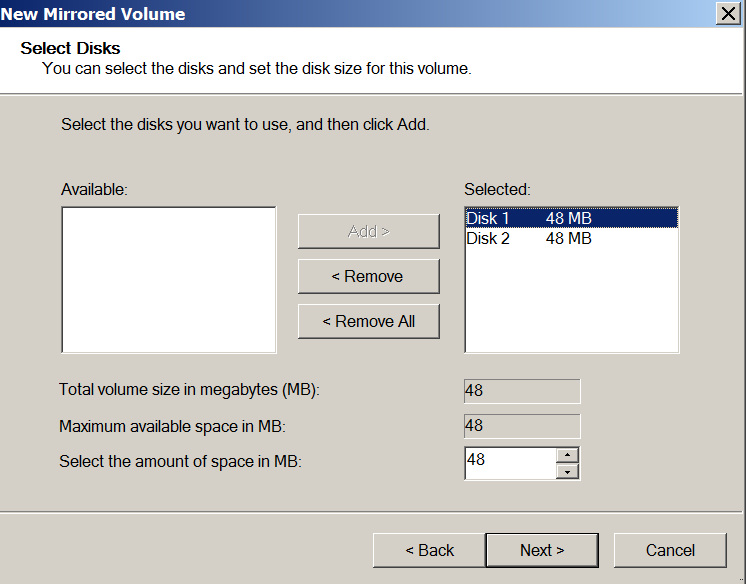
\includegraphics[scale=0.5]{raid4}
\caption{Añadimos ambos discos al RAID.}
\end{figure}
\begin{figure}[H]
\centering
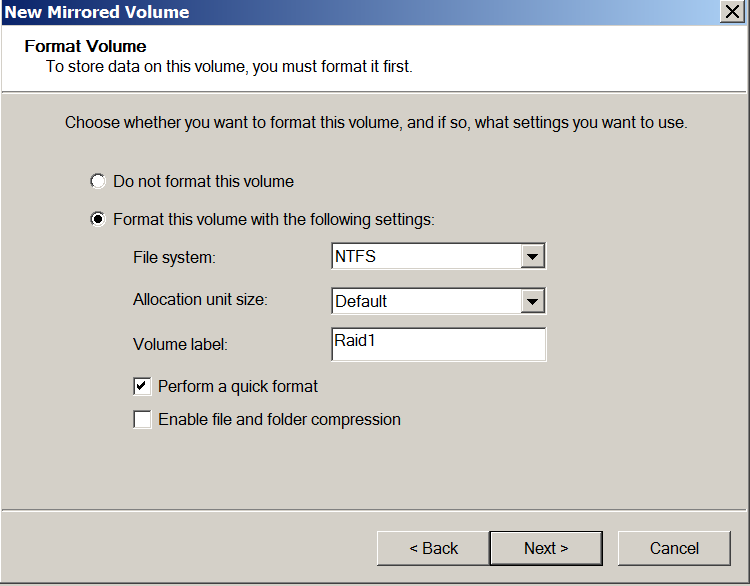
\includegraphics[scale=0.5]{raid5}
\caption{Elegimos el nombre y el sistema de archivos.}
\end{figure}
\begin{figure}[H]
\centering
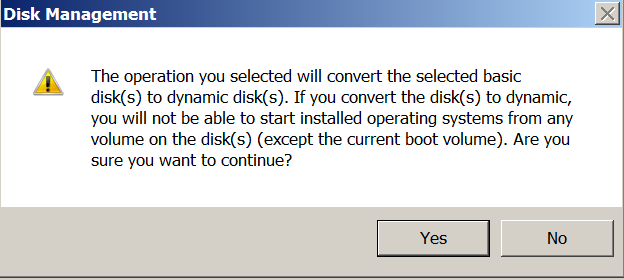
\includegraphics[scale=0.5]{raid6}
\caption{Aceptamos convertir los discos a dinámicos, ya que es necesario para montar un RAID.}
\end{figure}
\begin{figure}[H]
\centering
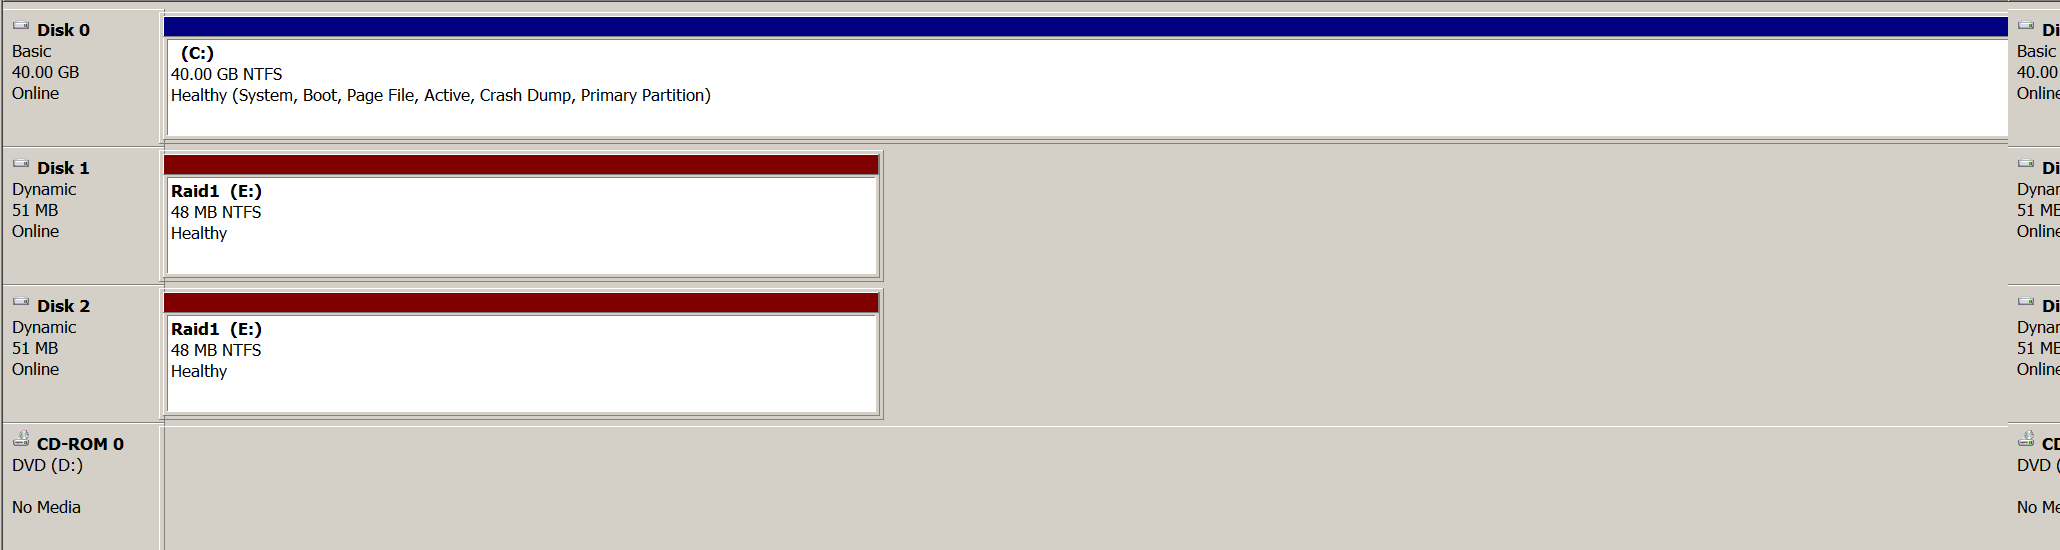
\includegraphics[scale=0.5]{raid7}
\caption{Como podemos observar, el RAID está en funcionamiento.}
\end{figure}


\section{Cuestión 16: Explique brevemente qué diferencias hay entre los tres tipos de conexión que permite el VMSW para las Mvs: NAT, Host-only y Bridge.}

El modo Bridge conecta a la máquina virtual directamente a la tarjeta de red del host se utiliza para máquinas que proveen servicios en internet, NAT asigna máquinas virtuales direcciones IP privadas dentro de la máquina física, pero comparten la misma dirección IP que el host en el exterior de la máquina física, por lo que está destinado a máquinas virtuales que necesitan acceso a la red, pero que no proporcionan servicios. Solo se podría acceder a la máquina virtual mediante reenvío de puertos NAT. Host-only no permite conexiones desde con las máquinas virtuales desde el exterior, conecta las máquinas virtuales host-only entre sí. Está diseñado para entornos de prueba aislados. \cite{25}

\newpage

\bibliography{P1-JorMacCan}
\bibliographystyle{ieeetr}

\end{document}